\chapter{PRINCIPLES OF DIFFERENTIAL PRIVACY}

During this chapter we are going to introduce the term of D.P., and its definition, alongside with the principles that need to be followed while applying it.

\section{Promise of Differential Privacy}

\par Differential Privacy is actually a promise made by the data handlers, to the participants of a study: "You will not be affected, adversely or otherwise, by allowing your data to be used in any study or analysis, no matter what other studies/ datasets/ info resources are available". 
\par The goal is to make the data widely available for analysis, while protecting the users. However, is it possible to learn nothing about an individual, while gathering useful information about a population? This is actually what D.P. is trying to achieve.


\section{Definition of Differential Privacy}
Before defining D.P., we must analyze some of the basic components of its definition.

\subsection{Randomized Response}
Randomized response is one of the earliest privacy mechanisms, that is used to conduct surveys where taboo behaviour is studied. The participants in those surveys are asked to answer truthfully, while they do not want to be stigmatized. There is a micro-world of what we are trying to achieve, thus we are going to give the algorithm of the randomized response in order to answer a binary (yes/no) question.

\begin{itemize}
    \item Flip a coin.
    \item If it lands on heads, answer truthfully
    \item If it lands on tails, flip another one
    \item If it lands on heads, answer no, else, answer yes
\end{itemize}

We are going to analyze this algorithm and its success in later chapters, but for now, it is enough to know that there exists a simple mechanism that adds noise, and is rather accurate for large samples.

Before giving the definition of D.P., we must define its components. 

\begin{itemize}
    \item \textbf{Probability Simplex}, given a discrete set $B$, is denoted as $\Delta(B)$ and is defined to be:
    \begin{align*}
        \Delta(B) = \{ x\in R^{|B|}: x_i \geq 0 \text { } \forall i \text{ and } \sum_{i=1}^{|B|} x_i = 1\}
    \end{align*}
    \item A \textbf {Randomized algorithm} $M$ with domain $A$ and discrete range of results $B$, is associated with the mapping $M: A\rightarrow\Delta(B)$. On
    \item \textbf{Distance between Databases:} The $l_1$ norm of a database x is denoted $||x||_1$ and it is defined to be: $||x||_1 = \sum_{i = 1}^{|x|} |x_i|$. Thus, the $l_1$ distance between 2 databases $x$ and $y$, is $||x-y||_1$, and the size of a database $x$ os $||x||_1$.
    
\end{itemize}
There are plenty definitions for D.P., but throughout this thesis we are going to use the one bellow.

\subsection{Definition}
Differential Privacy is defined as following:
\\
\\
A randomized algorithm $M$ with domain $N^{|x|}$ is (ε,δ)-differentially private, if for all $S \in Range(n)$ and for all $x,y \in N^{|x|}$ s.t. $||x - y||_1 \leq 1$
$$ Pr[M(x) \in S] \leq e^\epsilon Pr[M(y) \in S] + \delta$$

where the probability space is over the coin flips of the mechanisms $M$. If $\delta = 0$, we say that $M$ is ε-differentially private.

\\
It should be noted that D.P. is rather a definition than a strict algorithm. While relying on the definition of D.P., we can create different algorithms, which will all ensure that the result will be deferentially private. This allows us to create different forms of D.P., that will be analyzed later on this thesis.

The whole point of Differential Privacy, is that the output of a D.P. mechanism, should by \textbf{independent} of whether or not an individual is present in the domain $N$. The "ability" of the adversary to recognise the existence of a column in the dataset, is regularized by epsilon.

\section{The meaning of epsilon}
It is made clear from the above definition, that if we have a computational task, we might find different algorithms for applying D.P., but the result will always be of the same form: each user of the dataset, will get ε-D.P.. But what does the epsilon parameter actually mean?

By reading the mathematical equation, we observe that the higher the value of epsilon, the bigger the difference between the two probabilities (minimum and maximum). Thus, we extract the following statement about the value of epsilon during the application of Differential Privacy:

\begin{itemize}
    \item The \textbf{lower the epsilon} value, the \textbf{higher the privacy} guarantees for the users of the dataset.
    \item The \textbf{higher the epsilon} value, the \textbf{more accurate the results} produced.
\end{itemize}

In practice, epsilon values vary in the range $(0,5]$, as lower values are prohibited, and higher values are considered extreme cases. However, as mentioned in (TODO: Insert reference for Cynthia),  when epsilon is small, failing to be (ε,0)-differentially private is not necessarily alarming, if our algorithm is linearly increasing with ε (ex (2ε,0)-D.P). This happens because of the nature of the epsilon parameter, which guarantees very strict boundaries between databases. However, when ε increases by a lot, users' privacy suffers. 

In \textbf{Figure 2.1}, we can see in general terms, the function between the epsilon and the accuracy error, as well as the protection guaranteed. We will discuss in later sections the details on how these graphs are created, but now is a good time to get an overall picture of the accuracy error produced when applying D.P.
\bigskip
\bigskip\bigskip

\begin{figure}[!htb]\centering
      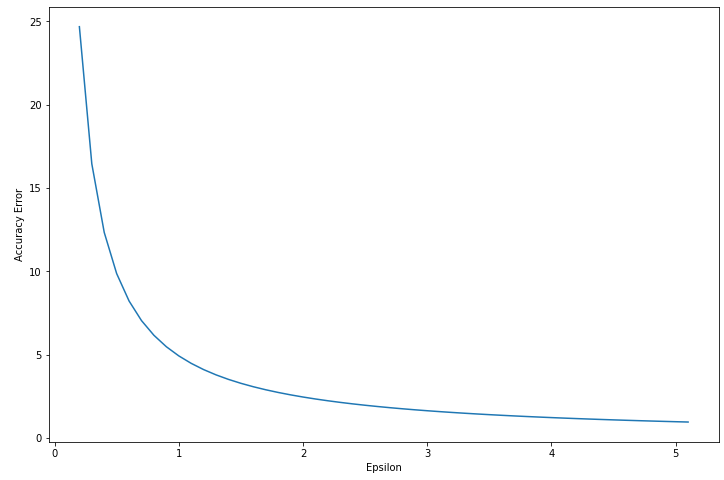
\includegraphics[width=0.6\textwidth]{images/epsilon_intro_graph.png}
  \caption{Accuracy Error as a function of epsilon}
\end{figure}

\section{Different forms of Differential Privacy}

As mentioned during the definition, due to the room that is left for its interpretation, there can be many forms of Differential Privacy. There are two major fields recognized, the \textbf{Global D.P.} and the \textbf{Local D.P.}.

Their major difference is the curator of the data. In the Global model, the curator must be trusted, as he collects the non-private data and has to pass them through a D.P. algorithm.

On the other hand, in the Local model, the curator may as well be untrusted, since the users perturb their data on their own, using a specific protocol. The key differences of the two forms are shown in the \textbf{Figure 2.2} below.

An other difference between the two models, is the amount of noise added. With the absence of a trusted curator, the users themselves must add a significant amount of noise into their data, in order to preserve their privacy. This of course results into a need of many users (several thousands), in order for the L.D.P. protocols to function correctly and accurately.


\begin{figure}[!htb]\centering
      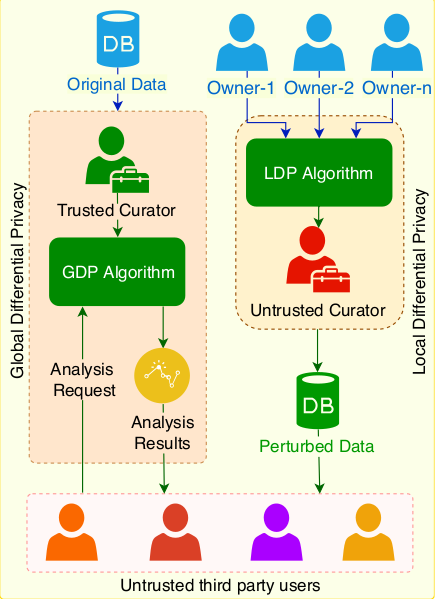
\includegraphics[width=0.3\textwidth]{images/local_vs_global.png}
  \caption{Differences between LDP and GDP}
\end{figure}

In this thesis, we are going to examine both models, by quoting their definitions, observing already-existing algorithms, and creating our own L.D.P. protocol.

\section{Existing Problems of D.P.}

As every new step in Computer Science, Differential Privacy has some issues that are yet to be solved, and some others not covered by its definition. 

One major problem is the behaviour of the protocols \textbf{when the number of users is limited}. The definition of D.P. is based on the alteration of the data in order not to reveal sensitive information. Thus, if a small amount of users are involved in those protocols, the accuracy of the results might be way off the standards that we set, in order to satisfy the epsilon requirements of the user.

Another (unsolvable) issue, that mainly lies on the basis of surveys, is  \textbf{the possibility that conclusions drawn from a survey may reflect statistical information about an individual}.

For example, if a survey about the correlation of smoking and dental problems is conducted, someone that has specific dental problems might be deemed as a smoker, despite keeping his privacy about the fact that he is smoking, during the survey. That is something that D.P. does not promise: unconditional freedom from distinguishing. This is not however a violation of the definition of D.P., as the survey teaches us that specific private attributes correlate with public observable attributes, since this correlation would be observed independent of the presence or absence of the individual in the survey.

There are several more issues as the ones covered above, however we are not going to focus on those, rather on the advantages of D.P.